% \begin{frame}{\large Research Objective: Rectification with Min. Topological Changes}
% \begin{figure}
% \centering
% 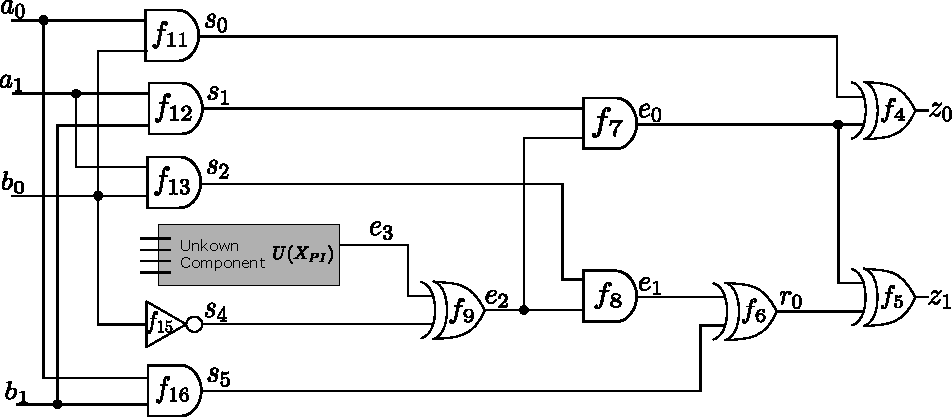
\includegraphics[scale=0.5]{mas_redundant_U.pdf}
% \end{figure}
% \bi
% 	\item In current formulation $U$ function of $X_{PI}$
% 	\item Disadvantage if net closer to PO
% 	\bi
% 		\item Re-synthesize significant portion of circuit
% 	\ei
% \ei
% \end{frame}

% \begin{frame}{\large Research Objective: Rectification with Min. Topological Changes}
% \begin{figure}
% \centering
% 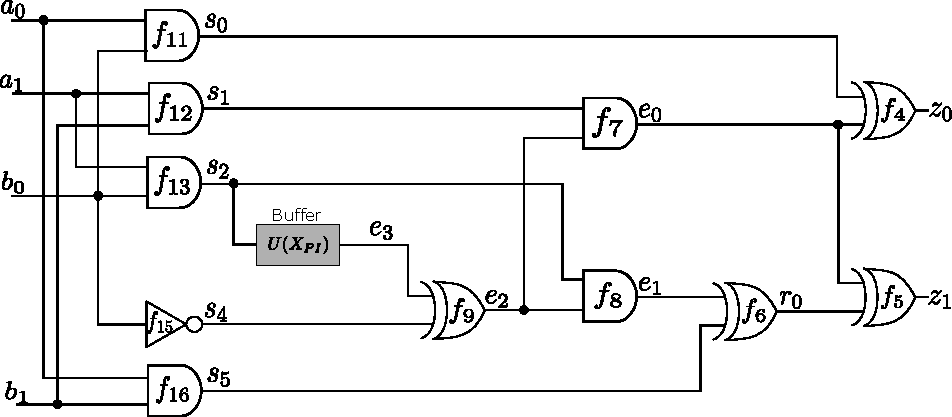
\includegraphics[scale=0.5]{mas_redundant_U_rewire.pdf}
% \end{figure}
% \bi
% 	\item Objective: Obtain $U$ in internal variables
% 	\bi
% 		\item Reuse already implemented logic
% 		\item Minimum (minimal) changes to the existing circuit
% 	\ei
% 	\item Approach: Different term orders for rectification formulation
% 	\bi
% 		\item Expensive GB computations in reduction procedures as RTTO $>$ is modified
% 	\ei
% \ei
% \end{frame}


% \begin{frame}{\large Research Objective: Integer arithmetic circuits}
% \begin{figure}[H]
%     \centering
%     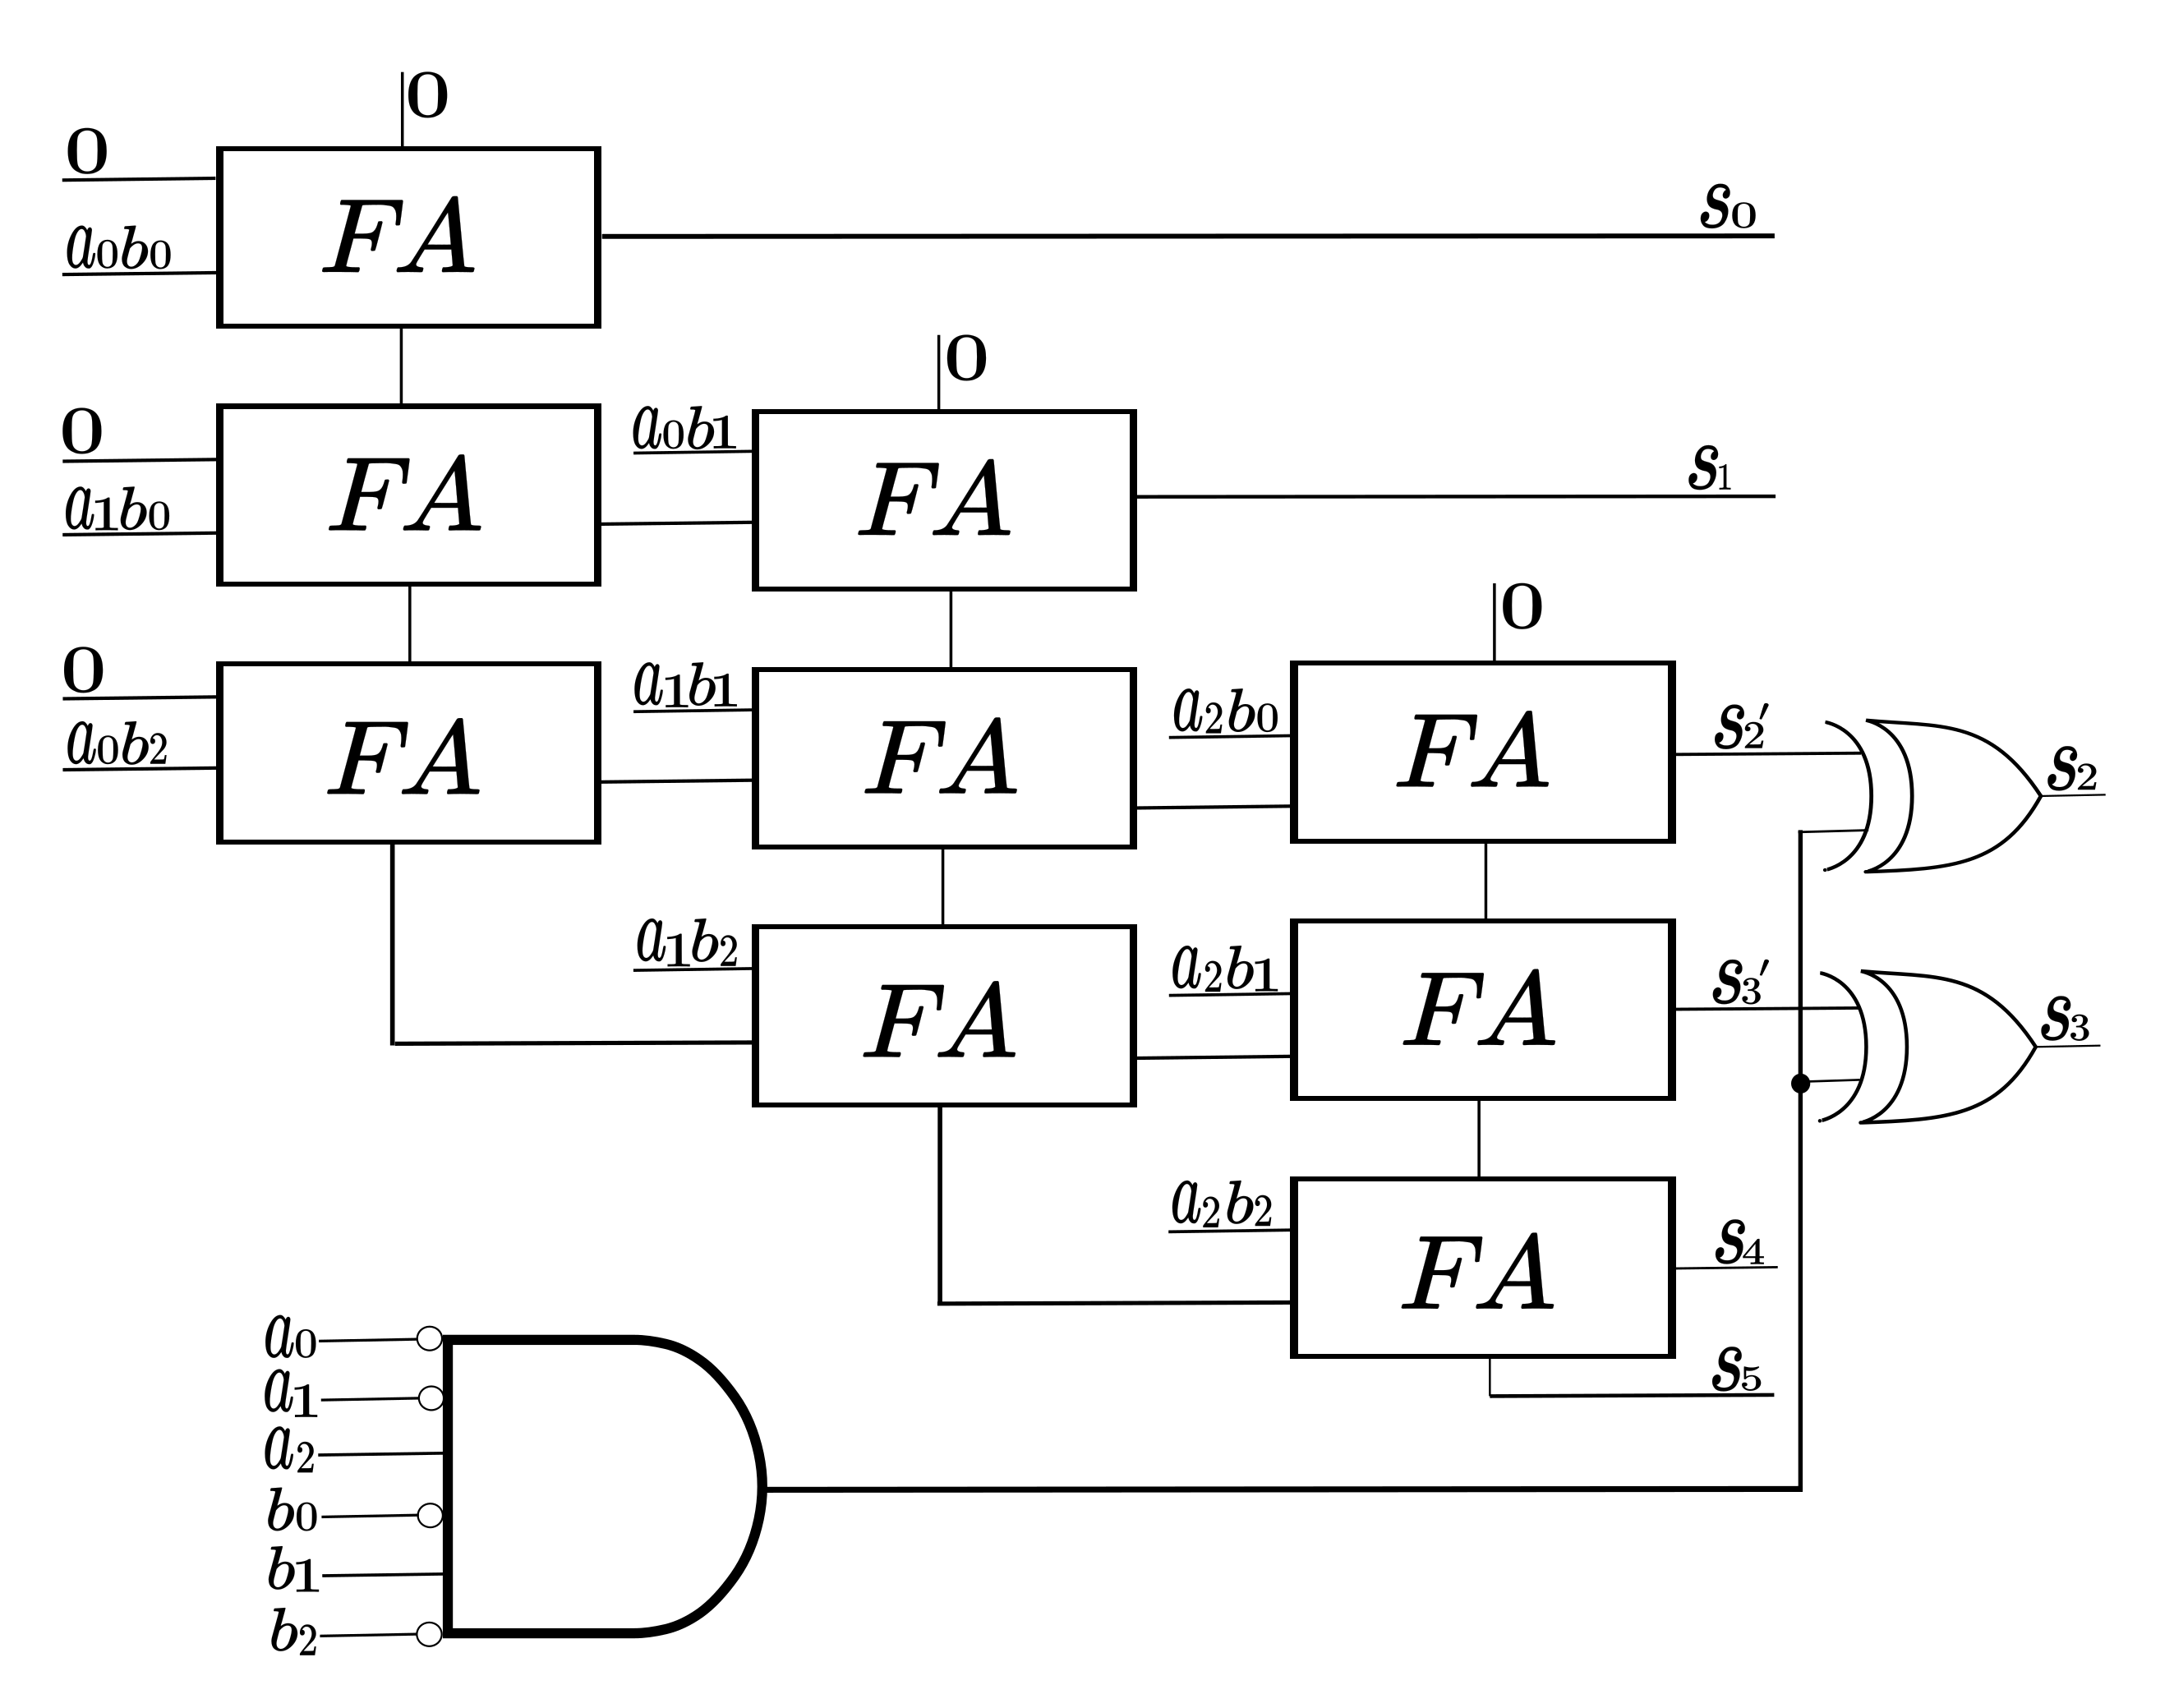
\includegraphics[scale = 0.07]{3appmult.png}
%     \caption{3-bit multiplier with additional circuit to introduce a bug}
%     \label{fig:3appmult}
% \end{figure}

% \end{frame}

% \begin{frame}{\large Research Objective: Integer arithmetic circuits}
% \bi
% 	\item Techniques valid over fields are inapplicable over rings
% 	\item \Grobner basis and division algorithms are complicated
% 	\item Can be modeled over $\Q$
% 	\bi
% 		\item Rectification function computation can result in {\it fractional coefficients}
% 		\item Extracting Boolean rectification function requires exhaustive simulation
% 		\item No scope of optimization as Extended \Grobner basis technique gives zero control
% 	\ei
% \ei

% \end{frame}

% \begin{frame}{\large Research Objective: Integer arithmetic circuits}


% {\tiny
% \begin{equation}
%     \begin{split}
% h_i & = 8\cdot a_0\cdot a_1\cdot a_2\cdot b_0
% +16\cdot a_0\cdot a_1\cdot a_2\cdot b_1
% -12\cdot a_0\cdot a_1 \\
% & -8\cdot a_0\cdot a_2\cdot b_0 
%  -16\cdot a_0\cdot a_2\cdot b_1 
%  +12\cdot a_0-8\cdot a_1\cdot a_2\cdot b_0 \\
% & -16\cdot a_1\cdot a_2\cdot b_1 
% +12\cdot a_1+8\cdot a_2\cdot b_0
% +16\cdot a_2\cdot b_1
% -12        
%     \end{split}
%     \nonumber
% \end{equation}

% \begin{equation}
%     \begin{split}
% h_i' = & -\frac{44}{3}\cdot a_0\cdot a_1\cdot a_2\cdot b_0\cdot b_1\cdot b_2+
% \frac{4}{3}\cdot a_0\cdot a_1\cdot a_2\cdot b_0\cdot b_1 \\
% & +8\cdot a_0\cdot a_1\cdot a_2\cdot b_0\cdot b_2
% +\frac{8}{3}\cdot a_0\cdot a_1\cdot a_2\cdot b_1\cdot b_2 \\
% & +\frac{4}{3} \cdot a_0\cdot a_1\cdot b_0\cdot b_1\cdot b_2
% -\frac{2}{3}\cdot a_0\cdot a_1\cdot b_0\cdot b_1 \\
% &+\frac{4}{3}\cdot a_0\cdot a_1\cdot b_1\cdot b_2
% +\frac{8}{3}\cdot a_0\cdot a_2\cdot b_0\cdot b_1\cdot b_2 \\
% & -4\cdot a_0\cdot a_2\cdot b_0\cdot b_2 
% +\frac{28}{3}\cdot a_1\cdot a_2\cdot b_0\cdot b_1\cdot b_2 \\
% & -\frac{14}{3}\cdot a_1\cdot a_2\cdot b_0\cdot b_1
% -\frac{8}{3}\cdot a_1\cdot a_2\cdot b_0\cdot b_2 \\
% &-\frac{20}{3}\cdot a_1\cdot a_2\cdot b_1\cdot b_2
% +\frac{8}{3}\cdot a_1\cdot a_2\cdot b_1 \\
% &-\frac{2}{3}\cdot a_1\cdot b_1 
% -\frac{4}{3}\cdot a_1\cdot b_2
% +1        
% \end{split}
% \nonumber
% \end{equation}}
% \end{frame}

% \begin{frame}{\large Research Objective: Integer arithmetic circuits}
% \begin{equation*}
%     r = -h_i'h_i+h_{i+1}'f_{i+1}+\dots+h_s'f_s+ \sum H_l' (x_l^2-x_l)
%     \label{eq:eqn6}
% \end{equation*}

% \vspace{2mm}
% \begin{table}[ht]
%     \centering
%     \begin{tabular}{|c|c|c|} \hline
%       $a_0,a_1,a_2,b_0,b_1,b_2$ & $h_i$ & $h_i'$ \\ \hline
%        0,0,0,0,0,0 & -12 & 1\\ \hline
%        0,0,0,0,0,1 & -12 & 1\\ \hline
%        0,0,0,0,1,0 & -12 & 1\\ \hline
%        0,1,0,0,0,1 & 0 & $-\frac{1}{3}$\\ \hline
%        0,1,0,0,1,0 & 0 & $\frac{1}{3}$\\ \hline
%        0,1,0,0,1,1 & 0 & -1 \\ \hline
%     \end{tabular}
%     \caption{Evaluating $h_i$ and $h_i'$}
%     \label{tab:quosol}
% \end{table}

% \bi
% 	\item Challenge: Formulating don't cares
% \ei

% \end{frame}

\begin{frame}{\large{Implementation: Boolean Polynomials and ZDDs}}
\bi
  \item Boolean polynomials as unate cube sets
  \bi
      \item Monomial: a product of positive literals or a cube
      \item Polynomial: set of such cubes
  \ei
  \pause
  \item ZDDs efficient for manipulating unate cube sets [Minato, DAC'93]
  \pause
  \item $r_1 = yd + y + d$ as $\{yd,y,d\}$
  % \item Cubes on ZDDs $\equiv$ Paths terminating in Node {\bf 1}
  % \item Solid edge implies variable present in cube 
\ei
\begin{figure}[hbt]
\centering
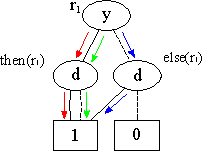
\includegraphics[scale=1.5]{r1_clean_paths.pdf}
\caption*{Paths terminating in 1: ${\color{red} yd}, {\color{green} y}, {\color{blue} d}  $.}
\label{r1}
\end{figure}
  
\end{frame}

\begin{frame}{\large{Improved Reduction Using ZDDs}}
\bi
  \item $r_1=yd + y + d$, $f_2=y + xc + x + c$, $r_1 \xrightarrow{f_2}_+$
  % \item $r_1 = yd + y + d$, ~~$f_2 = y + xc + x + c$
  % \item Quotient$(r_1 \xrightarrow{f_2}_+ r_2) = d+1$
  % \item $r_1 \xrightarrow{f_2}_+ r_2 = $
        {\small
        \begin{align*}
          & (yd + y + d) + (d + 1)\cdot(y + xc + x + c) \pmod{2}\\
          &= 2\cdot(yd + y) + d + (d+1)\cdot(xc + x + c) \pmod{2}\\
          &= \textcolor{green}{d} + (\textcolor{red}{d+1})\cdot(\textcolor{blue}{xc + x + c})  \pmod{2}
        \end{align*}
        }
  % \item This expression provides a formula to compute remainder in one step
\ei
\begin{figure}[hbt]
\centering
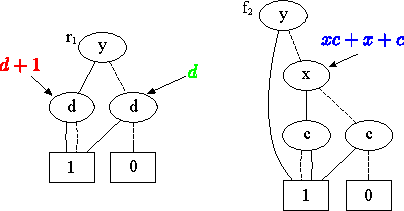
\includegraphics[scale=0.9]{r1_f2_2.pdf}
% \caption{ZDDs for polynomial $r_1$ and $f_2$.}
\label{f2}
\end{figure}
\bi
  \item One step reduction: $else(r_1) + then(r_1)\cdot else(f_2)$ ~~[Algorithm 6]
\ei
\end{frame}

\begin{frame}{\large Implementation}
\bi
	\item Custom software: 
	\bi
		\pause
		\vspace{0.1in}
		\item PolyBori reduction procedure for remainder generation
		\vspace{0.1in}
		\pause
		\item Singular to compute $P_k(x)$ and model composite field
		\vspace{0.1in}
		\pause
		\item Custom high level finite field engine 
		\pause
		\bi
		\item Bit-vector and coefficient computations
		\item Decision procedure
		\ei
	\ei
	\pause
	\item Experiments performed on a 3.5GHz 
	Intel(R) $\text{Core}^{\text{TM}}$ i7-4770K Quad-Core CPU with 32 GB RAM
\ei
\end{frame}

\begin{frame} {\large Overall Flow}


\end{frame}

\begin{frame}{\large MFR Experiments: Mastrovito}

% \begin{tiny}
% $\textit{n}$ = Datapath Size, $\textit{m}$ = target word size, 
% $\textit{k}$ = composite field size (degree of $P_k(X)$), 
% AM = Maximum resident memory utilization in Mega Bytes,
% \#G = Number of gates $\times 10^3$, \#BO = Number of faulty outputs, 
% PBS = Required time for PolyBori setup (ring declaration/poly collection/spec collection),
% VMS = Required time for verification, polynomial factorization and computing $P_k(X)$, and MFR setup, 
% RC = Required time for MFR check, TE = Required time for total execution
% \end{tiny}

{\scriptsize
\begin{table}[bht]
\centering
\caption*{{\scriptsize $\textit{n}$ = Datapath Size, $\textit{m}$ = target word size, 
$\textit{k}$ = composite field size (degree of $P_k(X)$),\\ 
AM = Maximum resident memory utilization in Mega Bytes,
\#G = Number of gates $\times 10^3$,\\ \#BO = Number of faulty outputs, 
PBS = Required time for PolyBori setup (ring declaration/poly collection/spec collection),
VMS = Required time for verification, polynomial factorization and computing $P_k(X)$, and MFR setup, 
RC = Required time for MFR check, TE = Required time for total execution}}
\label{masvsspec}
\begin{tabular}{| c | c | c | c | c | c | c | c | c | c |} \hline
{\textit{\textbf{n}}} & {\textit{\textbf{m}}} & {\textit{\textbf{k}}} & {\textbf{AM}} & {\textbf{\#G}} 
& {\textbf{\#BO}} & {\textbf{PBS}} & {\textbf{VMS}} & {\textbf{RC}} & {\textbf{TE}} \\ \hline 
16  & 5 & 80   & 100 & 0.8  & 6  & 0.04 & 0.06  & 0.12  & 0.22 \\ \hline
32  & 5 & 160  & 120 & 2.8  & 8  & 0.13 & 0.12  & 0.4   & 0.65 \\ \hline
163 & 5 & 815  & 550 & 69.8 & 6  & 6.04 & 3.36  & 11.9  & 21.3 \\ \hline
233 & 2 & 466  & 750 & 119  & 3  & 13   & 1.2   & 0.01  & 14.2 \\ \hline
283 & 2 & 566  & 1300& 190  & 2  & 38   & 4.2   & 0.1   & 42.3 \\ \hline
409 & 2 & 818  & 2400& 384  & 2  & 190  & 5     & 0.1   & 195  \\ \hline
\rowcolor{green}571 & 2 & 1042 & 5000& 827  & 5  & 2150 & 12    & 0.1   & 2162 \\ \hline
\end{tabular}
\end{table}}

\end{frame}

\begin{frame}{\large MFR Experiments: Montgomery}

{\scriptsize
\begin{table}[bht]
\centering
\caption*{{\scriptsize $\textit{n}$ = Datapath Size, $\textit{m}$ = target word size, 
$\textit{k}$ = composite field size (degree of $P_k(X)$), 
\\AM = Maximum resident memory utilization in Mega Bytes,
\#G = Number of gates $\times 10^3$, \\ \#BO = Number of faulty outputs, 
PBS = Required time for PolyBori setup (ring declaration/poly collection/spec collection),
VMS = Required time for verification, polynomial factorization and computing $P_k(X)$, and MFR setup, 
RC = Required time for MFR check, TE = Required time for total execution}}
\label{montvsspec}
\begin{tabular}{| c | c | c | c | c | c | c | c | c | c |} \hline
{\textit{\textbf{n}}} & {\textit{\textbf{m}}} & {\textit{\textbf{k}}} & {\textbf{AM}} & {\textbf{\#G}} 
& {\textbf{\#BO}} & {\textbf{PBS}} & {\textbf{VMS}} & {\textbf{RC}} & {\textbf{TE}} \\ \hline 
16  & 5 & 80   & 100 & 0.9  & 16  & 0.04 & 0.56 & 35.6     & 36   \\ \hline
32  & 5 & 160  & 120 & 2.8  & 32  & 0.13 & 0.57 & 27.6     & 28.3 \\ \hline
163 & 5 & 815  & 550 & 57.5 & 128 & 5.2  & 6.8  & 262      & 274  \\ \hline
233 & 2 & 466  & 750 & 112  & 233 & 11.5 & 3.5  & 360      & 375  \\ \hline
283 & 2 & 566  & 1300& 171  & 283 & 35   & 11   & 1503     & 1549 \\ \hline
\rowcolor{red}409 & 2 & 818  & 2400& 340  & 409 & 134  & 10   & 4920 & 5064 \\ \hline
\rowcolor{green}571 & 2 & 1042 & 5000& 663  &  12 & 1313 & 82   & 0.2 & 1395 \\ \hline
\end{tabular}
\end{table}}

\end{frame}

\begin{frame}{\large MFR Experiments: Point Addition}

{\scriptsize
\begin{table}[bht]
\centering
\caption*{{\scriptsize $\textit{n}$ = Datapath Size, $\textit{m}$ = target word size, 
$\textit{k}$ = composite field size (degree of $P_k(X)$), 
\\AM = Maximum resident memory utilization in Mega Bytes,
\#G = Number of gates $\times 10^3$, \\ \#BO = Number of faulty outputs, 
PBS = Required time for PolyBori setup (ring declaration/poly collection/spec collection),
VMS = Required time for verification, polynomial factorization and computing $P_k(X)$, and MFR setup, 
RC = Required time for MFR check, TE = Required time for total execution}}
\label{pavsspec}
\begin{tabular}{| c | c | c | c | c | c | c | c | c | c |} \hline
{\textit{\textbf{n}}} & {\textit{\textbf{m}}} & {\textit{\textbf{k}}} & {\textbf{AM}} & {\textbf{\#G}} 
& {\textbf{\#BO}} & {\textbf{PBS}} & {\textbf{VMS}} & {\textbf{RC}} & {\textbf{TE}} \\ \hline 
16 & 5 & 80   & 100 & 0.9  & 7   & 0.06 & 0.11 & 1.73 & 1.9  \\ \hline
32  & 5 & 160  & 120 & 2.9  & 13  & 0.18 & 0.8  & 134  & 135  \\ \hline
163 & 5 & 815  & 550 & 71.6 & 22  & 15.7 & 4.7  & 15   & 35.4 \\ \hline
233 & 2 & 466  & 750 & 122  & 233 & 19.2 & 2.15 & 0.15 & 21.5 \\ \hline
\rowcolor{green}283 & 2 & 566  & 1300& 208  & 4   & 80.4 & 6.1  & 0.1  & 86.6 \\ \hline
\rowcolor{red}409 & 2 & 818  & 2400& 368  & 409 & 220  & 10   & 2007 & 2237 \\ \hline
571 & 2 & 1042 & 5000& 813  & 5   & 2583 & 27   & 880  & 3490 \\ \hline
\end{tabular}
\end{table}}

\end{frame}



% {\tiny
% \begin{table}[]
% \centering
% \caption{{\footnotesize {\footnotesize Time is in seconds; $\textit{n}$ = Datapath Size, $\textit{m}$ = target word size, 
% $\textit{k}$ = composite field size (degree of $P_k(X)$), 
% AM = Maximum resident memory utilization in Mega Bytes,
% \#G = Number of gates $\times 10^3$, \#BO = Number of faulty outputs, 
% PBS = Required time for PolyBori setup (ring declaration/poly collection/spec collection),
% % VF = time for verification (Sec.~\ref{sec:verify}), MS = Multi-fix check setup time (Sec.~\ref{sec:comps} 
% % [Rectification Setup]), RC = time for MFR check (Thm.~\ref{Thm:rect}), TE = Total execution time.}}
% VMS = Required time for verification, polynomial factorization and computing $P_k(X)$, and MFR setup, 
% RC = Required time for MFR check, TE = Required time for total execution}}}
% \label{masusmontspec}
% \begin{tabular}{| c | c | c | c | c | c | c | c | c | c |} \hline
% {\textit{\textbf{n}}} & {\textit{\textbf{m}}} & {\textit{\textbf{k}}} & {\textbf{AM}} 
% & {\textbf{\#G}} & {\textbf{\#BO}} & {\textbf{PBS}} & {\textbf{VMS}} & {\textbf{RC}} & {\textbf{TE}} \\ \hline 
% \mb{16}  & \mb{5} & \mb{80  } & 100 & 0.9  & 7   & 0.06 & 0.11 & 1.73 & 1.9  \\ \hline
% \mb{32 } & \mb{5} & \mb{160 } & 120 & 2.9  & 13  & 0.18 & 0.8  & 134  & 135  \\ \hline
% \mb{64 } & \mb{3} & \mb{192 } & 160 & 10.6 & 64  & 0.84 & 0.56 & 58.1 & 59.5 \\ \hline
% \mb{96 } & \mb{2} & \mb{96  } & 240 & 24.8 & 96  & 2.46 & 0.64 & 14.9 & 18   \\ \hline
% \mb{128} & \mb{2} & \mb{128 } & 370 & 43.2 & 128 & 6.45 & 1.55 & 73   & 81   \\ \hline
% \mb{163} & \mb{5} & \mb{815 } & 550 & 71.6 & 22  & 15.7 & 4.7  & 15   & 35.4 \\ \hline
% \mb{233} & \mb{2} & \mb{466 } & 750 & 122  & 233 & 19.2 & 2.15 & 0.15 & 21.5 \\ \hline
% \mb{283} & \mb{2} & \mb{566 } & 1300& 208  & 4   & 80.4 & 6.1  & 0.1  & 86.6 \\ \hline
% \mb{409} & \mb{2} & \mb{818 } & 2400& 368  & 409 & 220  & 10   & 2007 & 2237 \\ \hline
% \mb{571} & \mb{2} & \mb{1042} & 5000& 813  & 5   & 2583 & 27   & 880  & 3490 \\ \hline
% \end{tabular}
% \end{table}}

% \end{frame}


% \begin{frame}{\large MFR Experiments: Custom software}

% {\tiny
% \begin{table}[]
% \centering
% \caption{{\footnotesize Time is in seconds; $\textit{I}$ = Index, $\textit{n}$ = Datapath Size, $\textit{m}$ = target word size, 
% $\textit{k}$ = composite field size (degree of $P_k(X)$), 
% AM = Maximum resident memory utilization in Mega Bytes,
% \#G = Number of gates $\times 10^3$, \#BO = Number of faulty outputs, 
% PBS = Required time for PolyBori setup (ring declaration/poly collection/spec collection),
% % VF = time for verification (Sec.~\ref{sec:verify}), MS = Multi-fix check setup time (Sec.~\ref{sec:comps} [Rectification Setup]), RC = time for MFR check (Thm.~\ref{Thm:rect}), TE = Total execution time.}}
% VMS = Required time for verification, polynomial factorization and computing $P_k(X)$, and MFR setup, 
% RC = Required time for MFR check, TE = Required time for total execution}}
% \label{mavsspec}
% \resizebox{\linewidth}{!}{
% \begin{tabular}{!{\vrule width 1pt} c | c | c | c | c !{\vrule width 1pt} c | c | c | c | c | c !{\vrule width 1pt} c | c | c | c | c | c !{\vrule width 1pt} c | c | c | c | c | c !{\vrule width 1pt}}\noalign{\hrule height 1pt}
% \multicolumn{5}{!{\vrule width 1pt} c !{\vrule width 1pt}}{} & \multicolumn{6}{ c !{\vrule width 1pt}}{Mastrovito} & \multicolumn{6}{ c !{\vrule width 1pt}}{Montgomery} & \multicolumn{6}{ c !{\vrule width 1pt}}{Point Addition}\\ \noalign{\hrule height 1pt}

% {\textit{I}} & {\textit{\textbf{n}}} & {\textit{\textbf{m}}} & {\textit{\textbf{k}}} & {\textbf{AM}} & {\textbf{\#G}} & {\textbf{\#BO}} & {\textbf{PBS}} & {\textbf{VMS}} & {\textbf{RC}} & {\textbf{TE}}& {\textbf{\#G}} & {\textbf{\#BO}} & {\textbf{PBS}} & {\textbf{VMS}} 
% & {\textbf{RC}} & {\textbf{TE}}& {\textbf{\#G}} & {\textbf{\#BO}} & {\textbf{PBS}} & {\textbf{VMS}} & {\textbf{RC}} & {\textbf{TE}}\\ \noalign{\hrule height 1pt}

% 1  & \mb{16}  & \mb{5} & \mb{80  } & 100 & 0.8  & 6  & 0.04 & 0.06  & 0.12  & 0.22 & 0.9  & 16  & 0.04 & 0.56 & 35.6     & 36   & 0.9  & 7   & 0.06 & 0.11 & 1.73 & 1.9  \\ \hline
% 2  & \mb{32 } & \mb{5} & \mb{160 } & 120 & 2.8  & 8  & 0.13 & 0.12  & 0.4   & 0.65 & 2.8  & 32  & 0.13 & 0.57 & 27.6     & 28.3 & 2.9  & 13  & 0.18 & 0.8  & 134  & 135  \\ \hline
% 3  & \mb{64 } & \mb{3} & \mb{192 } & 160 & 11.2 & 5  & 0.57 & 0.45  & 227   & 228  & 9.6  & 47  & 0.52 & 0.32 & 1.79     & 2.63 & 10.6 & 64  & 0.84 & 0.56 & 58.1 & 59.5 \\ \hline
% 4  & \mb{96 } & \mb{2} & \mb{96  } & 240 & 24.5 & 5  & 1.47 & 0.26  & 0.83  & 2.56 & 21   & 96  & 1.36 & 1.27 & 13.3     & 16   & 24.8 & 96  & 2.46 & 0.64 & 14.9 & 18   \\ \hline
% 5  & \mb{128} & \mb{2} & \mb{128 } & 370 & 43.2 & 5  & 3.23 & 0.5   & 2.03  & 5.76 & 35.8 & 128 & 2.8  & 1.4  & 64.2     & 68.4 & 43.2 & 128 & 6.45 & 1.55 & 73   & 81   \\ \hline
% 6  & \mb{163} & \mb{5} & \mb{815 } & 550 & 69.8 & 6  & 6.04 & 3.36  & 11.9  & 21.3 & 57.5 & 128 & 5.2  & 6.8  & 262      & 274  & 71.6 & 22  & 15.7 & 4.7  & 15   & 35.4 \\ \hline
% 7  & \mb{233} & \mb{2} & \mb{466 } & 750 & 119  & 3  & 13   & 1.2   & 0.01  & 14.2 & 112  & 233 & 11.5 & 3.5  & 360      & 375  & 122  & 233 & 19.2 & 2.15 & 0.15 & 21.5 \\ \hline
% 8  & \mb{283} & \mb{2} & \mb{566 } & 1300& 190  & 2  & 38   & 4.2   & 0.1   & 42.3 & 171  & 283 & 35   & 11   & 1503     & 1549 & 208  & 4   & 80.4 & 6.1  & 0.1  & 86.6 \\ \hline
% 9  & \mb{409} & \mb{2} & \mb{818 } & 2400& 384  & 2  & 190  & 5     & 0.1   & 195  & 340  & 409 & 134  & 10   & 4920*    & 5064 & 368  & 409 & 220  & 10   & 2007 & 2237 \\ \hline
% 10 & \mb{571} & \mb{2} & \mb{1042} & 5000& 827  & 5  & 2150 & 12    & 0.1   & 2162 & 663  &  12 & 1313 & 82   & 0.2$\td$ & 1395 & 813  & 5   & 2583 & 27   & 880  & 3490 \\ \hline\hline
% 11 & \mb{16}  & \mb{7} & \mb{112 } & 100 & 0.8  & 11 & 0.04 & 0.17  & 4.96  & 5.14 & 0.9  & 13  & 0.05 & 2    & 228      & 230  & 0.9  & 12  & 0.05 & 0.55 & 33   & 33.6 \\ \hline
% 12 & \mb{32 } & \mb{5} & \mb{160 } & 120 & 2.8  & 8  & 0.13 & 0.09  & 0.81  & 1.03 & 2.8  & 32  & 0.13 & 0.9  & 100      & 101  & 2.9  & 13  & 0.18 & 0.8  & 244  & 245  \\ \hline
% 13 & \mb{64 } & \mb{3} & \mb{192 } & 160 & 11.2 & 5  & 0.58 & 0.23  & 1.64  & 2.45 & 9.6  & 47  & 0.51 & 0.6  & 10.4     & 11.4 & 10.6 & 5   & 0.8  & 0.2  & 4    & 5 \\ \hline
% 14 & \mb{96 } & \mb{2} & \mb{96  } & 240 & 24.5 & 5  & 1.48 & 0.25  & 0.04  & 1.77 & 21   & 96  & 1.34 & 2.16 & 87.5     & 91   & 24.8 & 96  & 2.44 & 0.66 & 35.5 & 38.6 \\ \hline
% 15 & \mb{128} & \mb{2} & \mb{128 } & 370 & 43.2 & 5  & 3.21 & 0.53  & 0.1   & 3.84 & 35.8 & 128 & 2.7  & 1.3  & 66       & 70   & 43.2 & 128 & 6    &  2   & 73   & 81   \\ \hline
% 16 & \mb{163} & \mb{5} & \mb{815 } & 550 & 69.8 & 6  & 6.3  & 3.4   & 12    & 21.7 & 57.5 & 128 & 5.3  & 7.7  & 524      & 537  & 71.6 & 22  & 16   &  4.6 & 37   & 57.6 \\ \hline
% 17 & \mb{409} & \mb{2} & \mb{818 } & 2400& 384  & 2  & 208  & 4     & 0.03  & 212  & 340  & 13  & 127  & 7.9  & 0.13     & 135  & 368  & 3   & 210  &  8   & 928  & 1146 \\ \hline
% 18 & \mb{571} & \mb{2} & \mb{1042} & 5000& 827  & 5  & 2246 & 10    & 0.11  & 2256 & 663  & 427 & 1358 & 63.8 & 2.24     & 1424 & 813  & 5   & 2433 &  19  & 5    & 2457 \\ \noalign{\hrule height 1pt}
% \end{tabular}
% }
% \end{table}
% }
% \end{frame}

\begin{frame}{\large Conclusion and Future work}
\bi

	\item Algebraic approach for $m$-target MFR checking
	\bi
		\item Efficiency derived by interpreting targets as a bit-vector
	\ei
	\pause
	\item New mathematical insights for unified framework
	\bi
		\item Field incompatibility
		\item Primitive polynomial computation
	\ei
	\pause
	\vspace{0.1in}
	\vspace{0.1in}
	\item Computation of rectification function at the word-level
	\bi
		\item $W = a_2b_1b_2 + \beta \cdot a_2b_2$
		\item $r_3 = (a_2 \wedge b_1 \wedge b_2),~~rr_3 = (a_2 \wedge b_2)$
	\ei
	\pause
	\item Define and formulate existence of don't cares at the word-level
	\pause
	\item Extend the approach to integer arithmetic circuits
\ei
\end{frame}


% \begin{frame}{\large MFR Function Example}
% \bi
% 	\item Compute a rectification function of the form $W = U(X_{PI})$ 
% 	\bi
% 		% \item Here $U$ is the \textit{unknown component} computed as an $m$-bit-vector word
% 		\item $U(X_{PI}) = \sum_{i=0}^{m-1}\be^iu_i$ 
% 		\bi
% 			\item Where $u_i$'s represent the individual Boolean functions for the respective $w_i$'s.
% 		\ei
% 	\ei
% 	\pause
% 	\item A polynomial which can be computed to rectify the circuit
% 	\bi
% 		\item $W = a_2b_1b_2 + \beta \cdot a_2b_2$
% 		\item $r_3 = (a_2 \wedge b_1 \wedge b_2),~~rr_3 = (a_2 \wedge b_2)$
% 	\ei
% 	% \item The \textit{unknown component} problem is then formulated as an ideal membership test and
% 	% solved using extended \Grobner Basis: 
% 	% \begin{center}
% 	% 	\begin{align*}
% 	% 	&W + \be^0 e_0 + \be d_5  = W + U = W +\be^0(a_1b_2+a_2b_1)+\be a_2b_2;\\
% 	% 	&e_0 = a_1b_2+a_2b_1;~~d_5 = a_2b_2;
% 	% 	\end{align*}
% 	% \end{center}
% \ei
% \end{frame}


% \begin{frame}{\large Rectification function computation }

% \bi
% 	\item SFR of finite field arithmetic circuits
% 		[{\it Rao. et al}, FMCAD'18][{\it Rao. et al}, IWLS'18]
% 	\bi
% 		\item Quantification based computation
% 		\item Alternate to Craig Interpolation  
% 	\ei
% \vspace{0.1in}
% \item Currently addressing function computation at a word-level for finite field arithmetic circuits: 
% \bi
% \item Rectification function computation at multiple nets in terms of primary inputs [Due notification GLSVLSI'21]
% \bi
% 	% \item Synthesizing a correction function in terms of primary inputs 
% 	\item Define and formulate existence of don't cares 
% 	\item Devise algorithms to explore don't cares for logic optimization 
% \ei
% \item Formulate rectification setup in terms of internal nets of the circuit. 
% \bi
% 	\item Explore word-level don't care formulation in terms of internal nets.
% \ei
% \item Extend the multi-fix approach to integer arithmetic circuits and address the associated challenges.
% \ei
% \ei
% \end{frame}

% \begin{frame}{\large Objectives}
% \begin{enumerate}
% 	\item Enhance the investigations on MFR of finite field circuits to accommodate the following challenges 
% 	\vspace{0.1in}
% 	\bi
% 		\item Heuristics to identify effective rectification targets
% 		\vspace{0.1in}
% 		\item Rectification setup in terms of internal nets 
% 		\vspace{0.1in}
% 		\item Derive a word-level abstraction model
% 		\bi
% 			\item Address mathematical challenges posed by the word-level formulation
% 		\ei
% 		\vspace{0.1in}
% 		\item Define and formulate existence of don't cares at the word-level
% 		\vspace{0.1in}
% 		\item Devise algorithms to compute efficient low cost patch functions by exploring the don't care setup 
% 	\ei
% \end{enumerate}
% \end{frame}

% \begin{frame}{\large Objectives}
% \begin{enumerate}
% \setcounter{enumi}{1}
% 	\item Extension to integer arithmetic circuits
% 	\bi
% 		\item Formulate the MFR approach 
% 		\item Address the mathematical challenges associated with it  
% 	\ei
% 	\vspace{0.1in}	
% 	\item Improving scalability of the approach
% 	\bi
% 		\item Utilize PolyBori’s reduction procedure with ZDD data structure
% 		\item Develop a computational engine to implement the rectification framework
% 	\ei
% 	\vspace{0.1in}
% 	\item Theory of permissible functions [{\it Muroga. et al} ITC'89][{\it Fujita. et al} IWLS'19] 
% 	\bi
% 		\item Use don't cares for logic optimization
% 	\ei
% \end{enumerate}
% \end{frame}